\chapter{Wprowadzenie do tematyki pracy}
\label{cha:tematykaPracy}
Cyfrowa akwizycja obrazu pozwala na odwzorowanie widzialnej dla człowieka sceny w przestrzeni zdigitalizowanej. Takie przedstawienie obrazu umożliwia utrwalenie go na rozmaitych nośnikach pamięci i dostęp do niego w dowolnym momencie w przyszłości. Rejestrując zdjęcia z pewną częstotliwością i zachowaniem kolejności ich akwizycji otrzymuje się nagranie wideo. Pozwala ono śledzić zmiany na scenie następujące w czasie, takie jak ruch czy \textcolor{red}{zmiana} oświetlenia. Następujące po sobie obrazy zwane \textbf{ramkami} to \textbf{sekwencja wideo}.
\section{Podstawowe operacje i pojęcia towarzyszące przetwarzaniu obrazów}
Choć dla człowieka informacje zawarte na obrazie są proste w interpretacji, maszyna ''widzi'' ramkę jako zwykły ciąg liczb. Dlatego aby dokonywać automatycznej detekcji pewnych zjawisk i zależności, należy poddać ją odpowiednim przekształceniom, pozwalającym wyekstrahować interesujące powiązania. Często konieczna jest także zmiana sposobu reprezentacji pikseli. Równie ważne staje się również filtrowanie zakłóceń. W książce \cite{i1823330731} opisane są najczęściej wykorzystywane algorytmy używane w takim procesie. W tej sekcji omówione zostaną te z nich, które używane są przez niektórych twórców rozwiązań z rozdziałów \ref{cha:metodyStare} i \ref{cha:analiza}. 
\subsection{Filtracja}
Filtracja obrazu ma na celu wyeliminowanie niepożądanych cech obrazu. Jest to operacja kontekstowa, a więc wymagająca informacji o jasności piksela i jego otoczenia. Staje się przez to procesem wykorzystującym duże nakłady obliczeniowe maszyny, przez co znacznie opóźnia działanie metody wykorzystującej filtrację - dlatego też istotny jest dobór jak najbardziej optymalnego sposobu eliminacji zakłóceń w zależności od danych. Dostępnych jest wiele metod, jak choćby filtracja górno- lub dolnoprzepustowa czy filtracja medianowa. Dokonuje się także klasyfikacji filtrów na liniowe (w oparciu o kombinację wartości odpowiednich pikseli obrazu wejściowego) i nieliniowe (do przekształceń wykorzystujące nieliniową funkcję odpowiednich pikseli obrazu). 
\subsubsection{Filtr medianowy}
Najczęściej używaną metodą przy usuwaniu zakłóceń typu sól i pieprz (pojedynczych pikseli o bardzo niskim/wysokim poziomie jasności) jest filtracja medianowa. W przeciwieństwie do innych rozwiązań, dokonujących najczęściej rozmycia obrazu, pozwala ona na zachowanie kształtu widocznych na scenie obiektów. Dzieje się tak między innymi dlatego, iż nie wprowadza ona do obrazu żadnych nowych wartości. Oto przykład filtracji medianowej:
\begin{figure}[!htb]
\centering
$\begin{bmatrix}
    10 & 30  & 4 \\
    20 & \textbf{0}   & 5 \\
    0  & \textbf{190} & 22 \\
    20 & 50  & 20
\end{bmatrix}$ ,
$\begin{bmatrix}
    1 & 1 & 1 \\
    1 & 1 & 1 \\
    1 & 1 & 1
\end{bmatrix}$
$\Rightarrow$
$\begin{bmatrix}
    \mathrm{x} &  \mathrm{x}  & \mathrm{x} \\
    \mathrm{x} & 10 & \mathrm{x} \\
    \mathrm{x} & 20 & \mathrm{x} \\
    \mathrm{x} &  \mathrm{x}  & \mathrm{x} 
\end{bmatrix}$
\caption{Przykładowa filtracja medianowa. Po lewej - wartości wejściowe, na środku okno filtracji, po prawej - wynik. Ponieważ operacja uwzględnia wartości sąsiedztwa, piksele brzegowe, które nie mogą być przefiltrowane w prosty sposób, oznaczone zostały jako x.}
\end{figure}
Jak widać, ponieważ pogrubione piksele reprezentowały skrajne jasności w swoim sąsiedztwie (w tym przypadku $3\times 3$), zostały podmienione wartościami mediany ze zbioru pikseli otoczenia. Wykorzystując tę metodę można odszumić nawet skrajnie zakłócony obraz. Należy jednak pamiętać, iż nadaje się ona głównie do eliminowania artefaktów typu sól i pieprz. Pozostawia także po sobie ślady w postaci ''obgryzionych'' krawędzi - niekiedy zmniejszając bądź zwiększając obszar zajmowany przez obiekty. Ważnym jest więc dobór odpowiedniego rozmiaru sąsiedztwa - większe okno wiąże się ze skuteczniejszą eliminacją zakłóceń, jednak mocno zniekształca obraz. Zwiększają się także wymagania algorytmu w kwestii obliczeniowej.
\subsection{Dylatacja}
Jednym z podstawowych przekształceń morfologicznych, czyli modyfikujących rozmiar i kształt figury na obrazie, jest dylatacja. Najczęściej wykonywana jest na obrazie binarnym. Ma ona na celu ''powiększanie'' elementów, często w celu rekonstrukcji bądź uwydatnienia pewnych ich cech.
\paragraph{}
Do wykonywania tej operacji służy \textbf{element strukturalny}, czyli pewien fragment obrazu z wyróżnionym punktem centralnym. Jest on przesuwany po całym obrazie w celu sprawdzania zgodności wzorca, a następnie podejmowana jest decyzja co do nowej wartości piksela centralnego. Jeśli którykolwiek z pikseli branych pod uwagę na podstawie szablonu elementu strukturalnego ma wartość '1', w przypadku dylatacji piksel centralny również otrzymuje wartość '1'.
\begin{figure}[!htb]
\centering


\includegraphics[width=0.4\textwidth]{img/sample}

\includegraphics[width=0.4\textwidth]{img/sample}
\caption{Dylatacja z obiektem strukturalnym 3x3. Po lewej - wejściowy obraz, po prawej - obraz po dylatacji}
\end{figure}
\subsection{Erozja}
Erozja jest niejako operacją przeciwną do dylatacji. 
%Operacją wykorzystywaną przy filtrach liniowych jest splot funkcji, czyli konwolucja. Ponieważ reprezentacja obrazów w przestrzeni cyfrowej jest dyskretna, również operacja splotu, w przestrzeni liczb rzeczywistych definiowana jako całka, może być opisana za pomocą zwykłego równania sumy:
%\begin{equation}
%\label{eq:konwolucja}
%L'(m,n) = (w x L)(m,n) = \sum_{i,j \in K} L(m-i, n-j)w(i,j)
%\end{equation}
%, gdzie L - obraz wejściowy, L' - efekt splotu obrazu z maską konwolucji, w - maska konwolucji, (m, n) - współrzędne piksela, dla którego wykonywana jest konwolucja jego otoczenia z maską w.\\
%Przykładowy splot fragmentu obrazu z maską filtru uśredniającego 3x3:
%\begin{equation}
%\label{eq:konwolucjaPrzyklad}

%\end{equation}
%\subsubsection{Normalizacja}
%Ponieważ w konwolucji wykonywane są operacje mnożenia i dodawania, otrzymane wartości mogą znacznie wykraczać poza zakres, jaki należy uzyskać w danej przestrzeni - najczęściej powinna być to liczba z przedziału [0, 255]. Jak łatwo zauważyć, w przykładzie \ref{eq:konwolucjaPrzyklad} tak właśnie się stało. W celu dostosowania uzyskanych liczb do wymaganego zakresu dokonuje się normalizacji. Jeśli w masce obecne są wyłącznie elementy nieujemne, każdy wynik konwolucji dzielony jest przez sumę jej elementów. Jeśli jednak współczynniki w macierzy w są zarówno dodatnie, jak i ujemne, normalizacja musi odbywać się według następującego wzoru:
%\begin{equation}
%L''(m,n) = \dfrac{L'(m,n)-minL'(m,n)}{maxL'(m,n)-minL'(m,n)}
%\end{equation}
\subsection{Przestrzenie barw}
\label{sec:colorSpace}
Przestrzeń barw to pewna matematyczna reprezentacja światła widzialnego w przestrzeni cyfrowej. W zależności od potrzeb stosowane są różne modele. Najpopularniejszymi są spotykane w urządzeniach elektronicznych trójkanałowe RGB (ang. \textit{Red Green Blue}) oraz komplementarny do niego, stosowany w druku CMYK (ang. \textit{Cyan Magenta Yellow blacK}), wykorzystujące właściwości ludzkiego wzroku determinujące sposób, w jaki człowiek odbiera barwy. Każdemu pikselowi obrazu są tu przypisane odpowiednie wartości na każdym kanale, na przykład czerwony piksel w reprezentacji RGB na kanale czerwonym (R) ma maksymalną wartość 255 (w 8-bitowej głębi kolorów), na niebieskim i zielonym po 0. Stosowane są one do łatwej do interpretacji przez człowieka reprezentacji cyfrowej kolorów na zdjęciach. Wprowadzają one jednak duże ograniczenia ze względu na ilość niesionej informacji. Akwizycja obrazu w innej przestrzeni pozwala na przykład na zastosowanie o wiele szerszego spektrum barw. Dlatego też często przy przetwarzaniu obrazów stosuje się inne modele, rozdzielające istotne dla maszyny informacje na oddzielne kanały, co umożliwia wydajniejsze i niekiedy dokładniejsze obliczenia na zdjęciach.
\paragraph{}
\begin{figure}[!htb]
\centering
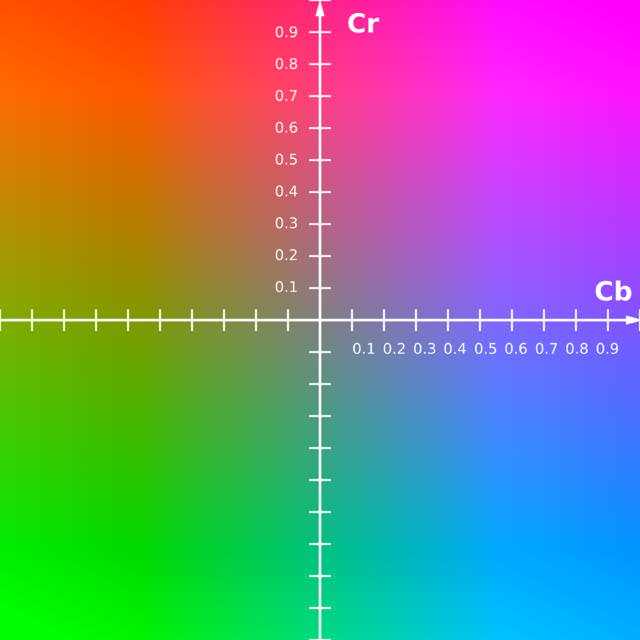
\includegraphics[width=182px]{img/YCbCr}
\caption{Reprezentacja płaszczyzny 
CbCr dla stałej luminancji Y=0.5}
%\floatfoot{Source: Wikipedia}
\end{figure}
W metodzie opisanej w rozdziale \ref{sec:BinWang}  używana jest przestrzeń YCbCr, oddzielająca kanał luminancji (Y), czyli poziomu jasności piksela, od kanałów chrominancji (Cb i Cr), przechowujących informację o jego odcieniu i nasyceniu. Taki sposób reprezentacji powstał z wykorzystaniem faktu, iż oko ludzkie jest o wiele bardziej czułe na poziom jasności obiektu, niż na jego kolor. Konwersja z przestrzeni RGB do YCbCr jest stosunkowo prosta - można ją zapisać w postaci macierzy:
%\begin{equation}

\[
\begin{bmatrix}
    Y & Cb & Cr \\
\end{bmatrix}
=
\begin{bmatrix}
    R & G & B \\
\end{bmatrix}
\begin{bmatrix}
    0.299 & -0.168935 & 0.499813 \\
    0.587 & -0.331665 & -0.418531 \\
    0.114 & 0.50059 & -0.081282 
\end{bmatrix}
\]

%\end{equation}

Ponieważ wartości na kanałach RGB mieszczą się w przedziale 0-255, po przekształceniu do przestrzeni YCbCr otrzymujemy odpowiednio wartości z przedziału [0, 255] na kanale Y oraz [-128, 127] na kanałach Cb i Cr.
\section{Analiza obrazu}  
%\subsection{Binaryzacja}
%Jest to jedna z podstawowych metod punktowego przetwarzania obrazu.  Pozwala odseparować istotne informacje na zdjęciu z pominięciem zależności mniej interesujących, takich jak na przykład konkretny poziom jasności, utrudniających tylko dalsze przetwarzanie ze względu na większą złożoność obliczeń. Obraz zostaje sprowadzony do postaci binarnej (zero-jedynkowej), gdzie najczęściej (w zależności od podejścia) 0 reprezentuje tło, 1 - interesujący obszar obrazu.  
%\paragraph{}
%Istnieje wiele metod binaryzacji, dlatego też można wybrać odpowiednią dla każdego algorytmu. Podstawowym problemem staje się jednak wyznaczenie odpowiedniego progu binaryzacji - ze względu na następującą w procesie radykalną redukcję informacji zawartych w obrazie, źle dobrany graniczny poziom jasności może doprowadzić do błędnej detekcji, w konsekwencji skutkującej złym działaniem programu. Dlatego też bardzo ważna jest znajomość rodzaju danych, z jakimi system przetwarzający będzie miał do czynienia - pozwoli to zastosować odpowiednią dla nich metodę obliczenia progu.
\subsection{Segmentacja obiektów}
Celem każdej segmentacji jest otrzymanie binarnej, czarno-białej reprezentacji, na której wyekstrahowane zostały interesujące fragmenty obrazu wejściowego - na przykład obiekty w ruchu bądź na pierwszym planie. Choć częściej segmentacja służy do przygotowania informacji zawartych na zdjęciu do dalszej analizy - jak choćby pomiarom czy śledzeniu obiektów w przypadku sekwencji wideo, uzyskane w ten sposób wyniki mogą być końcową fazą działania algorytmu. Istnieje wiele metod segmentacji, od binaryzacji z wykorzystaniem arbitralnie dobranego progu dla całego obrazu, poprzez rozrost, zalewanie obszaru i wiele innych. Bardzo ważnym jest dobór odpowiedniego sposobu w zależności od danych, z jakimi algorytm będzie miał do czynienia. Zły dobór metody może prowadzić do błędnych, a często nawet i bezużytecznych wyników - binaryzacja z globalnym progiem przy nierównomiernym oświetleniu często nie potrafi sobie poradzić z wyekstrahowaniem tekstu pisanego.
\begin{figure}[!htb]
\centering


\includegraphics[width=0.4\textwidth]{img/sample}

\includegraphics[width=0.4\textwidth]{img/sample}
\caption{Przykładowa segmentacja. Po lewej - ramka z nagrania, po prawej wynik segmentacji}
\end{figure}

\paragraph{}
Segmentacja obiektów pierwszoplanowych staje się szczególnie trudnym zagadnieniem w przypadku detekcji ruchu na scenie. O ile uzyskanie informacji o obiekcie przemieszczającym się przeważnie nie jest skomplikowane, utrzymanie modelu pierwszego planu dla elementów zatrzymanych nastręcza już sporych trudności. Spowodowane jest to koniecznością dostosowywania modelu tła do panujących warunków, przez co statyczne obiekty mogą ulegać błędnej inkorporacji do tego modelu.
\section{Detekcja ruchu na scenie}
Detekcja ruchu, czyli \textit{Motion Detection}, to sposób wykrywania przemieszczania się obiektów na scenie względem ich sąsiedztwa. Polega ona na analizie kolejnych ramek z sekwencji wideo i badaniu zmian następujących pomiędzy nimi.
\paragraph{}
Ze względu na trudność problemu detekcji, opracowanych zostało wiele metod odseparowania obiektów poruszających się od statycznych elementów sceny. Jedną z nich, stosunkowo najprostszą, jest odjęcie od obrazu wejściowego modelu uzyskanego przy pomocy algorytmów generacji tła. Na tym etapie twórcy metod muszą rozważyć jednak trzy podstawowe kwestie:
\begin{itemize}
\item czym jest model i jak się zachowuje?
\item jak dokonać inicjalizacji modelu tła?
\item w jaki sposób aktualizować model w czasie?
\end{itemize}
Związane jest to z faktem, iż bardzo rzadko na sekwencjach wideo rejestrowane są sytuacje idealne - często scenie towarzyszą zmiana oświetlenia (zwłaszcza w długotrwałym monitoringu na zewnątrz) lub szumy/zakłócenia, czego rezultatem jest, iż pomimo braku ruchu obiektów poszczególne piksele zmieniają swoją wartość - co przy standardowym podejściu polegającym na porównaniu wartości pikseli odpowiadających sobie pomiędzy ramkami skutkuje fałszywą detekcją. Rzadko również do dyspozycji są sekwencje z "czystym" obrazem tła - na próbkowanych ramkach znajdują obiekty już w ruchu, albo statyczne, jednak mogące w każdej chwili zmienić swoje położenie - jak choćby zaparkowane samochody. Zasłaniają one tło, przez do wygenerowanie prawidłowego modelu staje się bardzo trudne, a niekiedy niemożliwe. Opisane w dalszej części rozwiązania stworzone zostały z uwzględnieniem niniejszych ograniczeń.
\subsection{Modelowanie tła}
Jednym z najczęściej używanych w detekcji ruchu na scenie rozwiązań pośrednich jest modelowanie tła. Polega ono na stworzeniu modelu referencyjnego sceny bez żadnych ruchomych obiektów, co pozwala na późniejsze porównanie z nim kolejnych ramek nagrania w celu wykrycia zmian. Najczęściej odbywa się to poprzez algorytmy subtrakcji tła - obliczana jest absolutna różnica pomiędzy modelem tła a aktualnie analizowanym obrazem sceny, co skutkuje otrzymaniem obrazu, na którym niezerowe wartości są interpretowane jako obiekty pierwszoplanowe.
\paragraph{}
W rzeczywistości jednak to zagadnienie okazuje się być o wiele bardziej skomplikowane. W nagraniach rejestrowanych przez kamery w monitoringu wizyjnym rzadko dostępny jest materiał, na którym widoczne jest samo tło. Usuwanie wszelkich obiektów ze sceny i trenowanie maszyn monitorujących za każdym razem, kiedy tło zmieni się - na przykład zostanie wybudowany nowy budynek bądź nastąpi przemeblowanie wewnątrz pomieszczenia - jest bardzo uciążliwe. Twórcy oprogramowania zajmującego się automatyczną detekcją obiektów borykają się także z problemami, jakich nastręcza zjawisko ruchu obrotowego Ziemi - zmiennym oświetleniem sceny w zależności od pory dnia. Trzeba bowiem brać pod uwagę, iż na obrazie reprezentowana jest jasność poszczególnych pikseli - im mniej światła, tym ciemniejsze stają się obiekty. Można pomyśleć, iż ta kwestia rozwiązana zostać może poprzez zmianę przestrzeni kolorów i odseparowanie luminancji pikseli od ich barwy (\ref{sec:colorSpace}), jednak i tu pojawiają się problemy - mniej światła oznacza dużo mniej dokładną akwizycję barwy piksela, a co za tym idzie mogą pojawiać się różnice odcieni w czasie. Występuje tu analogia do procesu widzenia człowieka - oko ludzkie potrafi rozpoznawać kształt i ruch nawet przy bardzo słabym oświetleniu, odbywa się to jednak kosztem postrzegania w kolorze. W półmroku człowiek rejestruje więc otoczenie w skali szarości.
\paragraph{}
Z tych i wielu innych powodów zagadnienie modelowania tła staje się kluczowym w przypadku wielu algorytmów. Dobry obiekt referencyjny pozwala bowiem na ograniczenie detekcji do zwykłego porównywania wartości poszczególnych pikseli. Najczęściej proces modelowania odbywa się na podstawie początkowej sekwencji testowej, a następnie wzorzec tła jest uaktualniany poprzez odpowiednie modyfikacje przez cały czas działania programu wykrywającego ruch. Stosowanych jest wiele podejść, wykorzystujących zarówno proste mechanizmy, jak średnia wartość piksela na obrazie, jak i nieco bardziej zaawansowane, oparte na statystyce i probabilistyce. Warto wspomnieć tu o modelach gaussowskich, pojawiających się w większości proponowanych obecnie rozwiązań. Zasada ich działania opisana zostanie w dalszej części pracy.
\paragraph{}
Standardowe podejścia w dziedzinie generacji tła, jak średnia jasność bądź model Gaussa na podstawie pojedynczej ramki, nie dają jednak spodziewanych rezultatów w przypadkach obecności drobnego ruchu na scenie. Obiekty tła pozostające w ciągłym \textcolor{red}{ruchu} mogą bowiem przyjmować diametralnie skrajne wartości jasności. Posiadanie więc jednego modelu tła okazuje się nie być wystarczające. Te same algorytmy dla różnych zestawów nagrań wykazują się odmienną skutecznością, co jest zjawiskiem niepożądanym - dobry system detekcji powinien pracować prawidłowo niezależnie od panujących warunków.
\begin{figure}[!htb]
\centering


\includegraphics[width=0.4\textwidth]{img/sample}

\includegraphics[width=0.4\textwidth]{img/sample}
\caption{Modelowanie tła. Po lewej - ramka z nagrania, po prawej wyidealizowany model tła}
%\floatfoot{Source: }
\end{figure}
\subsection{Metody uaktualniania modelu tła}
Aby utrzymać prawidłową pracę systemu detekcji w zmiennych warunkach, należy dokonywać uaktualniania modelu tła na bieżąco. Polega to na podmianie wartości niektórych pikseli modelu bardziej \textcolor{red}{aktualnymi}. Ze względu na politykę stosowaną w tym procesie wyróżniane są dwie metody:
\begin{itemize}
\item konserwatywna
\item ślepa
\end{itemize} 
Metoda \textbf{konserwatywna} (ang. \textit{conservative update}) polega na uaktualnianiu wartości tylko dla tych pikseli, które zaklasyfikowane zostały obecnie jako tło. Choć z pozoru najbardziej intuicyjna, może doprowadzić do poważnych problemów na przykład przy błędnej detekcji elementów tła - jeśli nieprawidłowo wykryto ruch, nie będzie możliwe uaktualnianie modelu dla fałszywie sklasyfikowanych pikseli. Prowadzi to do powstawania tak zwanych \textbf{duchów} (ang. \textit{ghosts}) - efektów błędnej detekcji, które są propagowane w dalszym procesie działaniu algorytmu. Alternatywą dla tego sposobu jest metoda \textbf{ślepa} (ang. \textit{blind update}). Choć zapobiega zakleszczeniom, które mogą zdarzyć się przy polityce konserwatywnej, daje bardzo słabe wyniki dla obiektów poruszających się wolno, jako że piksele uaktualniane są niezależnie od tego, do którego modelu zostały przydzielone.

%\section{Standardowe metody a dynamiczne tło}
\section{Narzędzia}
\subsection{Język C++}
\subsection{Biblioteka OpenCV}

OpenCV (ang. \textit{Open Source Computer Vision}) to dostępna od 2000 roku biblioteka, zawierająca implementacje najczęściej wykorzystywanych algorytmów wizyjnych. Jej główne zalety to dostępność na zasadach \textit{open source}, a także wieloplatformowość. Została ona napisana w języku C, jednak istnieją specjalne nakładki, pozwalające korzystać z niej także m. in. w C++, C\#, Python i języku Java. Udostępniony publicznie jest nie tylko kod źródłowy, ale także i narzędzia, pozwalające na samodzielną kompilację biblioteki, co pozwala na używanie jej w wielu środowiskach programistycznych.
\paragraph{}
Biblioteka ta zawiera ponad 2500 algorytmów zoptymalizowanych pod względem pamięciowym i obliczeniowym. Jest ciągle rozwijana, co pozwala domniemywać, iż zawarte w niej rozwiązania pozwalają maksymalnie wykorzystać możliwości sprzętowe obecnych urządzeń. Korzystanie z niej zdaje się więc być najbardziej odpowiednie dla problemu opisywanego w niniejszej pracy, jako że szybkość przetwarzania wideo jest kluczowa dla detekcji w czasie rzeczywistym.
\begin{figure}[!htb]
\centering


\includegraphics[width=82px]{img/ocv_logo}
\caption{Logo biblioteki OpenCV \cite{OpenCVLogo}}
%\floatfoot{Source: }
\end{figure}

Do rozwiązania problemu rozważanego w tej pracy użyta została biblioteka \textbf{OpenCV 2.4.9}, dostępna od 25.04.2014r.